\section{Discussion}
\subsection{Parsimony and Physical Interpretability Are Prevalent Across Models}
Interestingly, our findings reveal a trend that contrasts with observations reported in some prior studies\cite{DONG2024130941,ZHOU2024132235}, where increased model complexity has been associated with improved predictive performance. As shown in Table~\ref{tab:complexity}, models with higher predictive skill (NSE $\geq$ 0.5) exhibit significantly lower structural complexity compared to lower-performing counterparts, as indicated by a reduced number of nodes (45.77 vs. 56.35, $p = 5.00 \times 10^{-5}$). This suggests that increased model complexity does not necessarily translate into improved performance in this context; instead, more parsimonious architectures may facilitate better generalization\cite{ORTH2015147}. One possible explanation is that overly complex models introduce redundant representations or noise, which can degrade predictive robustness in hydrological applications\cite{Wrr_PGDL}.

Several factors may explain why additional complexity can reduce performance in this setting. First, a larger circuit can absorb site-specific noise and transient correlations, which weakens out-of-sample robustness under hydro-climatic variability. Second, when many correlated predictors are represented through redundant internal paths, the model may dilute dominant controls (e.g., precipitation-state coupling) across multiple weak pathways, reducing effective signal-to-noise ratio. Third, in sparse-training regimes, over-parameterized structures increase optimization burden and make it harder to isolate a stable core predictive subnetwork, so pruning removes less redundancy and retains more unstable interactions. Collectively, these effects can produce a complexity penalty rather than a complexity benefit.

\begin{table}[htbp]
    \centering
    \caption{Structural complexity across NSE-based performance groups}
    \begin{tabular*}{\textwidth}{@{\extracolsep{\fill}}lccc}
        \toprule
        Group & Stations & Mean Nodes & Median Nodes \\
        \midrule
        NSE $<$ 0.5    & 194 & 56.35 & 56.50 \\
        NSE $\geq$ 0.5 & 327 & 45.77 & 42.00 \\
        All            & 521 & 49.71 & 49.00 \\
        \bottomrule
    \end{tabular*}

    \vspace{3pt}
    \begin{minipage}{\textwidth}
        \footnotesize
        \textit{Note:} A statistically significant difference is observed between groups ($p = 5.00 \times 10^{-5}$).
    \end{minipage}
    \label{tab:complexity}
\end{table}

From the perspective of physical interpretability, the probe analysis (Table~\ref{tab:probe}) indicates that key hydrological variables—including CUM, API, and CHG consistently encoded in the learned representations across models\cite{pmlr-v97-verma19a}. Specifically, no statistically significant differences are observed in probe performance between NSE-based groups (all $p > 0.05$). This implies that the ability to capture physically meaningful signals is not restricted to high-performing models\cite{e24050687_Shap_problem}, but rather is a common characteristic across the model population.

\begin{table}[htbp]
    \centering
    \begin{threeparttable}
        \caption{Probe performance under different NSE conditions}
        \begin{tabular*}{\textwidth}{@{\extracolsep{\fill}}llccc}
            \toprule
            Probe & Group & Mean & Median & p-value \\
            \midrule

            \multirow{3}{*}{$R^2_{\mathrm{cum}}$}
            & NSE $<$ 0.5    & 0.8746 & 0.9639 & \multirow{3}{*}{0.4341} \\
            & NSE $\geq$ 0.5 & 0.8915 & 0.9617 & \\
            & All            & 0.8851 & 0.9621 & \\

            \midrule

            \multirow{3}{*}{$R^2_{\mathrm{api}}$}
            & NSE $<$ 0.5    & 0.8795 & 0.9682 & \multirow{3}{*}{0.5676} \\
            & NSE $\geq$ 0.5 & 0.8917 & 0.9651 & \\
            & All            & 0.8871 & 0.9663 & \\

            \midrule

            \multirow{3}{*}{$R^2_{\mathrm{chg}}$}
            & NSE $<$ 0.5    & 0.3791 & 0.4267 & \multirow{3}{*}{0.1563} \\
            & NSE $\geq$ 0.5 & 0.4054 & 0.4406 & \\
            & All            & 0.3955 & 0.4342 & \\

            \bottomrule
        \end{tabular*}

        \begin{tablenotes}
            \footnotesize
            \item Outliers were excluded using the 1.5 IQR criterion within each group. Results remain consistent without filtering.
        \end{tablenotes}
        \label{tab:probe}
    \end{threeparttable}
\end{table}

Taken together, these results suggest that parsimony and physical interpretability are not competing objectives. Instead, models with simpler structures are capable of achieving strong predictive performance while still encoding essential hydrological knowledge related to streamflow generation. This result motivates the next question: \textit{if such knowledge is broadly present across models, what is its concrete content and spatial organization across basins?}

\FloatBarrier

\subsection{Learned Core Circuits Reflect Hydrological Knowledge Across Basins}

\begin{figure*}[htbp]
    \centering
    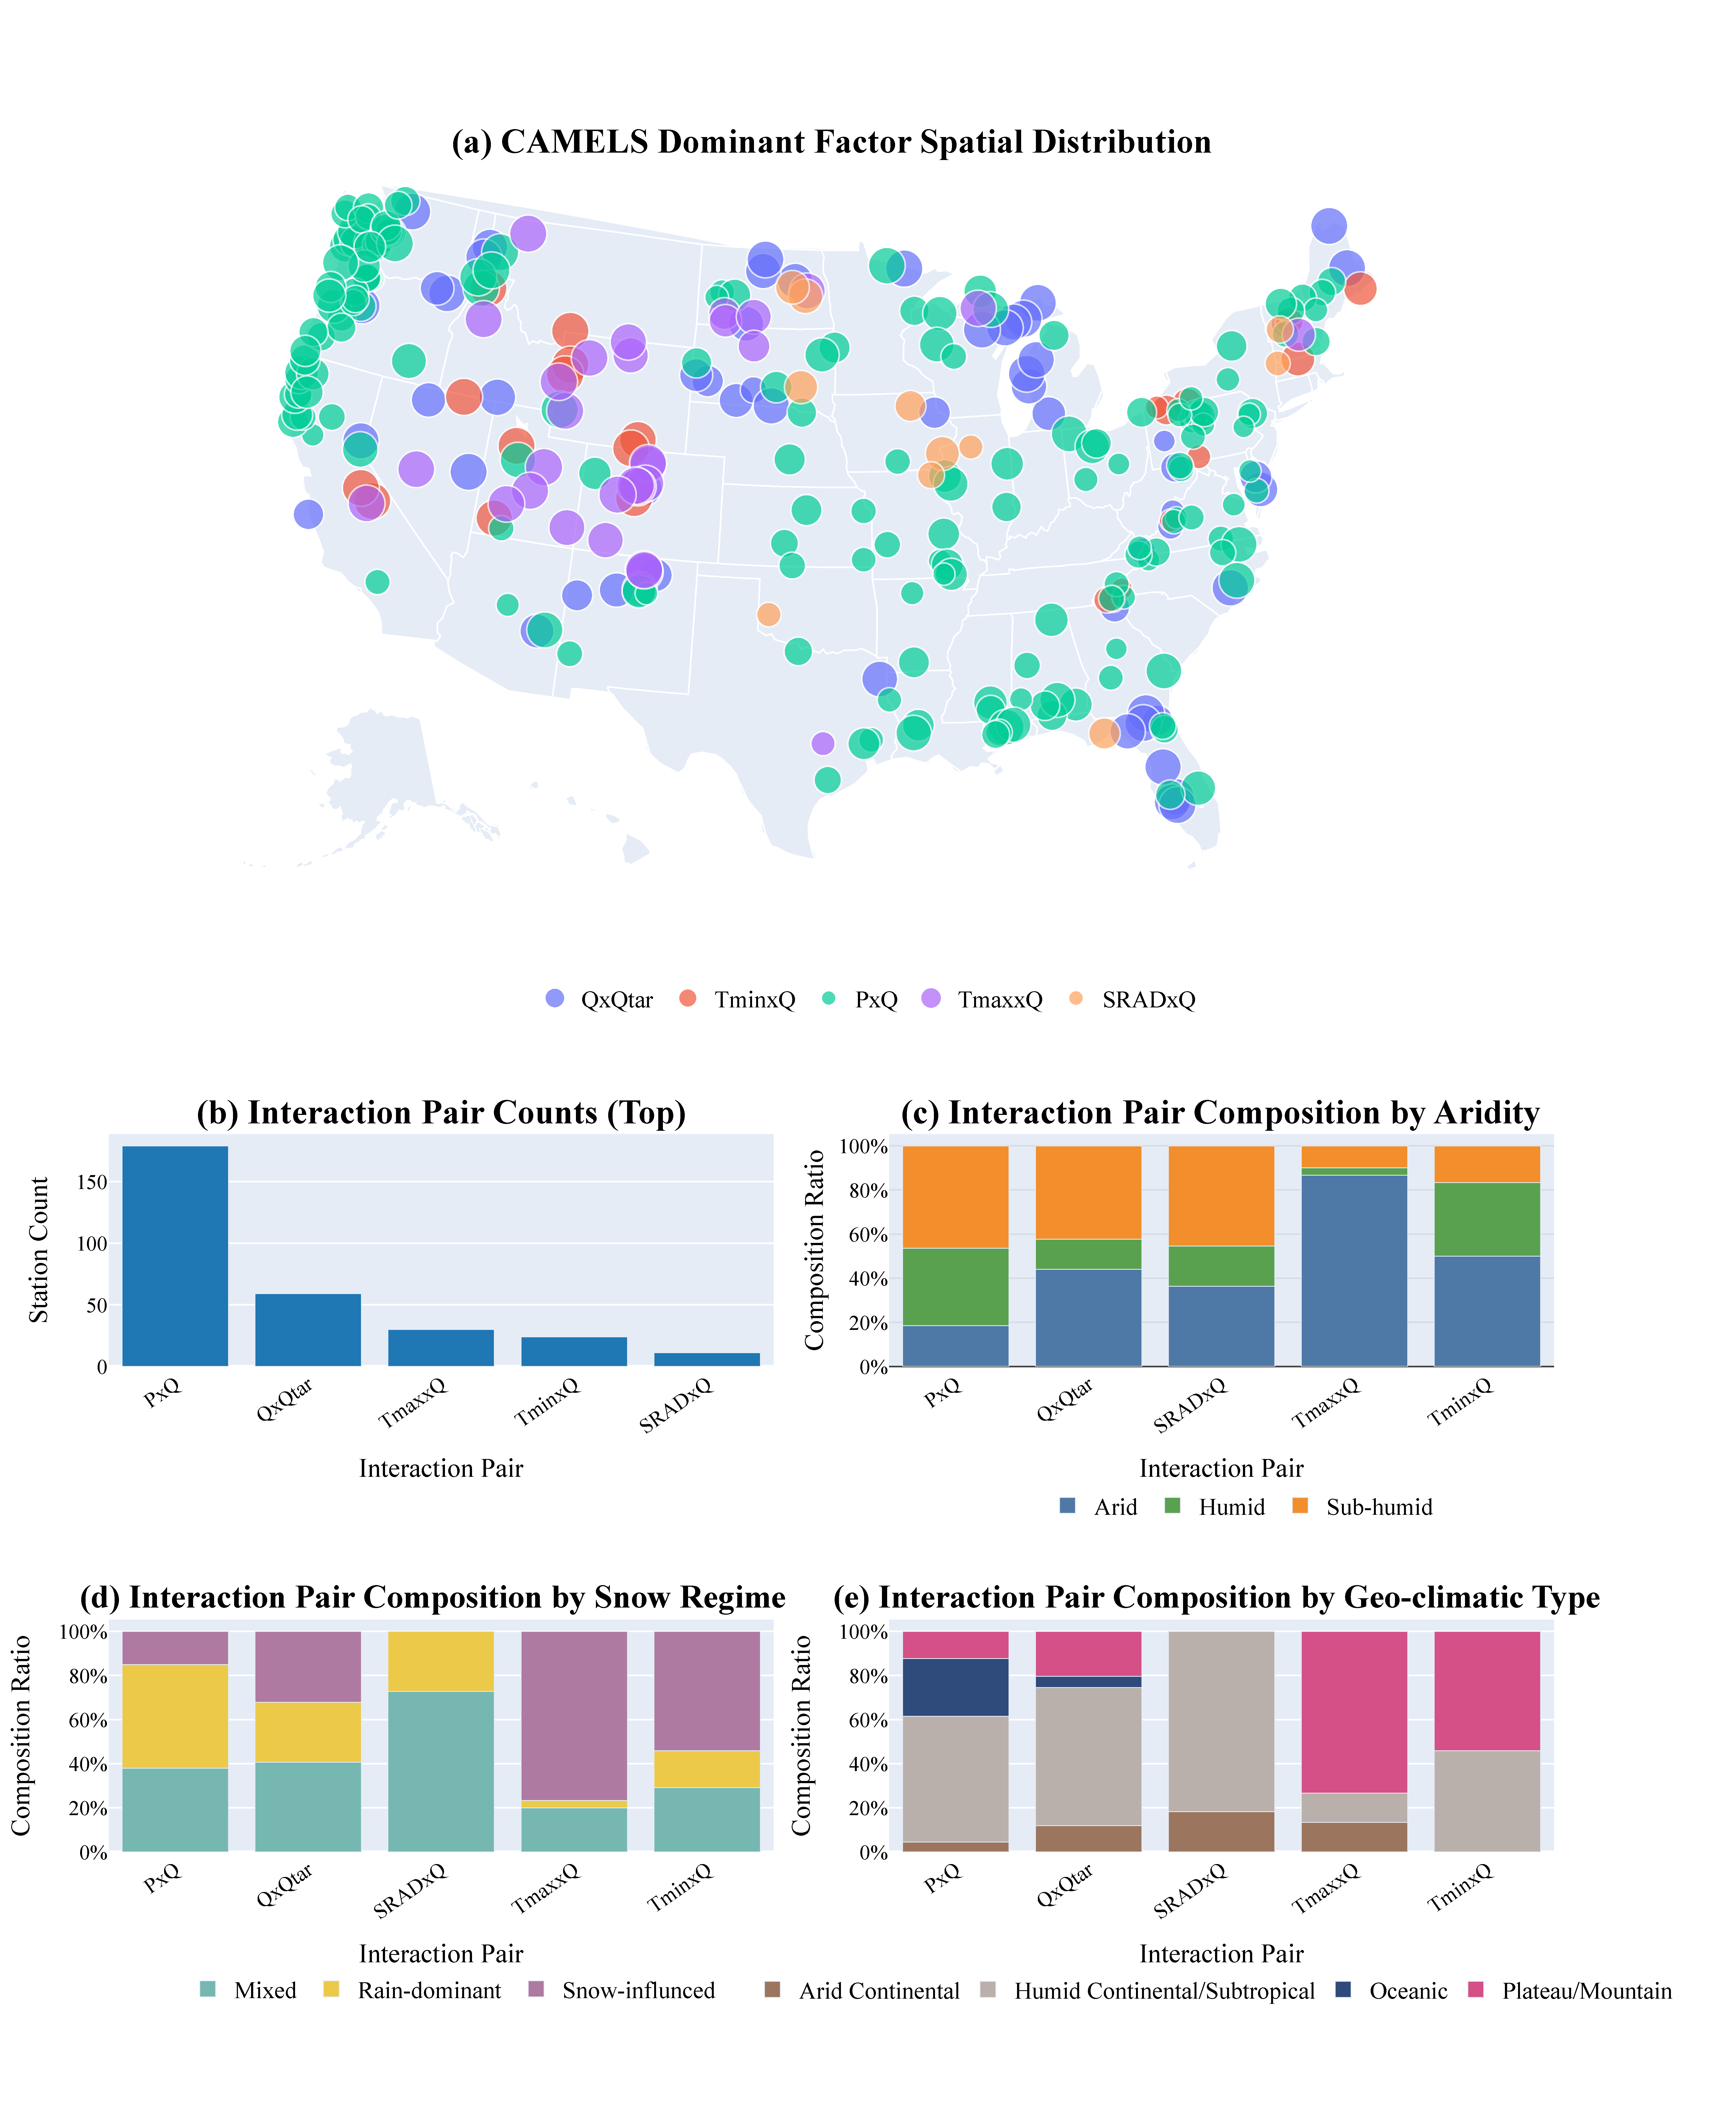
\includegraphics[width=\textwidth]{Figures/interaction_analysis.pdf}
    \caption{(a) Spatial distribution of dominant interaction factors across basins. (b) Frequency of top interaction pairs. (c) Interaction composition under different aridity conditions. (d) Interaction composition across snow regimes. (e) Interaction composition across geo-climatic types.}
    \label{fig:interaction_analysis}
\end{figure*}

To answer that question, we examine the spatial organization of the learned core interaction circuits. The results show that the model captures structured and regime-dependent hydrological knowledge across diverse basins\cite{hess-camels}. As shown in Fig.~\ref{fig:interaction_analysis}(a), the dominant interaction in most basins is between precipitation and discharge (P--Q), reflecting the fundamental role of precipitation as the primary driver of streamflow generation\cite{Berghuijs2014}. Importantly, this is not only a feature-attribution result; it indicates a recurrent hydrological mode in which rainfall forcing dominates the event-scale runoff pathway across many catchments. The detailed procedure for how we performed the classification can be found in the Supplementary Information~\ref{sec:knowledge}.

In contrast, a subset of basins is characterized by strong interactions between lagged discharge and target discharge (Q--Q$_{\mathrm{target}}$), suggesting pronounced memory effects\cite{apak2026multi}. In these basins, streamflow dynamics are more strongly influenced by antecedent conditions than by immediate precipitation inputs, which is typically associated with limited precipitation or strong storage capacity. This pattern can be interpreted as a storage-controlled response mode, where antecedent wetness and catchment retention regulate subsequent flow release.

Temperature-related interactions (T$_{\max}$--Q and T$_{\min}$--Q) are primarily observed in inland and high-elevation regions. These patterns indicate that temperature plays a critical role in regulating streamflow generation in such environments, not only through snowmelt processes but also via evaporation and other energy-limited controls\cite{milly2020colorado}. In addition, interactions involving shortwave radiation (SRD) emerge in some basins, further highlighting the importance of energy inputs\cite{immerzeel2010climate} in modulating hydrological responses. Together, these signals correspond to an energy-constrained runoff mode, distinct from precipitation-dominated systems.

These patterns remain consistent across different hydro-climatic conditions, as illustrated in Fig.~\ref{fig:interaction_analysis}(b--e). Precipitation-driven interactions dominate across most basins, whereas temperature-related and lagged discharge interactions become more prominent under specific environmental settings. In arid and semi-humid regions, temperature and memory-related interactions are more frequently observed\cite{milly2020colorado}, indicating stronger energy constraints and persistence effects. In contrast, humid basins are largely governed by precipitation-driven dynamics\cite{Berghuijs2014}.

Similarly, temperature-related interactions\cite{immerzeel2010climate} are concentrated in snow-influenced basins, consistent with snowmelt-controlled streamflow processes, while precipitation-driven interactions dominate in rain-fed systems\cite{Wrr_p_q}. Across different geo-climatic types, distinct interaction circuits exhibit clear regional preferences, suggesting that the learned structures adapt to local environmental conditions.

Overall, these findings demonstrate that the learned core circuits are not arbitrary but systematically reflect regime-dependent hydrological patterns\cite{hess-24-1081-2020}. Thus, STEH moves the interpretation target from "which variable is important" to "which process pathway is operating," providing structural evidence that the model internalizes physically meaningful knowledge beyond simple variable associations. However, structural coherence alone is insufficient: the extracted knowledge should also produce physically consistent behavior under controlled perturbations.

\subsection{Accurate Volume Response but Limited Sensitivity to Temporal and State Perturbations}

Following the structural analysis above, we next test whether the extracted hydrological knowledge corresponds to realistic model behavior. As shown in Fig.~\ref{fig:counterfactual_main}, the counterfactual analysis reveals that the model exhibits physically meaningful responses under different types of perturbations\cite{read2019process}. For magnitude-based interventions, particularly rainfall scaling (Fig.~\ref{fig:counterfactual_main}b), the model produces directionally consistent and approximately linear changes in streamflow volume across stations. As precipitation increases (or decreases), the predicted streamflow volume correspondingly increases (or decreases), while prediction error remains largely unchanged. This indicates that the model has successfully learned a stable and physically consistent mapping between precipitation and streamflow generation, allowing it to respond reliably to changes in input water magnitude without compromising predictive accuracy\cite{nearing2021role}.

Under rainfall pattern redistribution (Fig.~\ref{fig:counterfactual_main}c), the total precipitation is conserved, and the predicted streamflow volume remains largely stable, consistent with mass conservation expectations\cite{WRR_NSE}. However, structural differences emerge across redistribution modes. In particular, under the back-loaded configuration, a noticeable increase in streamflow volume is observed. This suggests that the model is sensitive to the temporal concentration of rainfall and produces stronger streamflow responses\cite{hess-camels} when precipitation is concentrated toward later periods, reflecting an initial capability to capture rainfall-streamflow lag relationships. Meanwhile, the variation in prediction error across scenarios indicates that the model's utilization of temporal structure remains somewhat scenario-dependent.
\begin{figure}[ht]
    \centering
    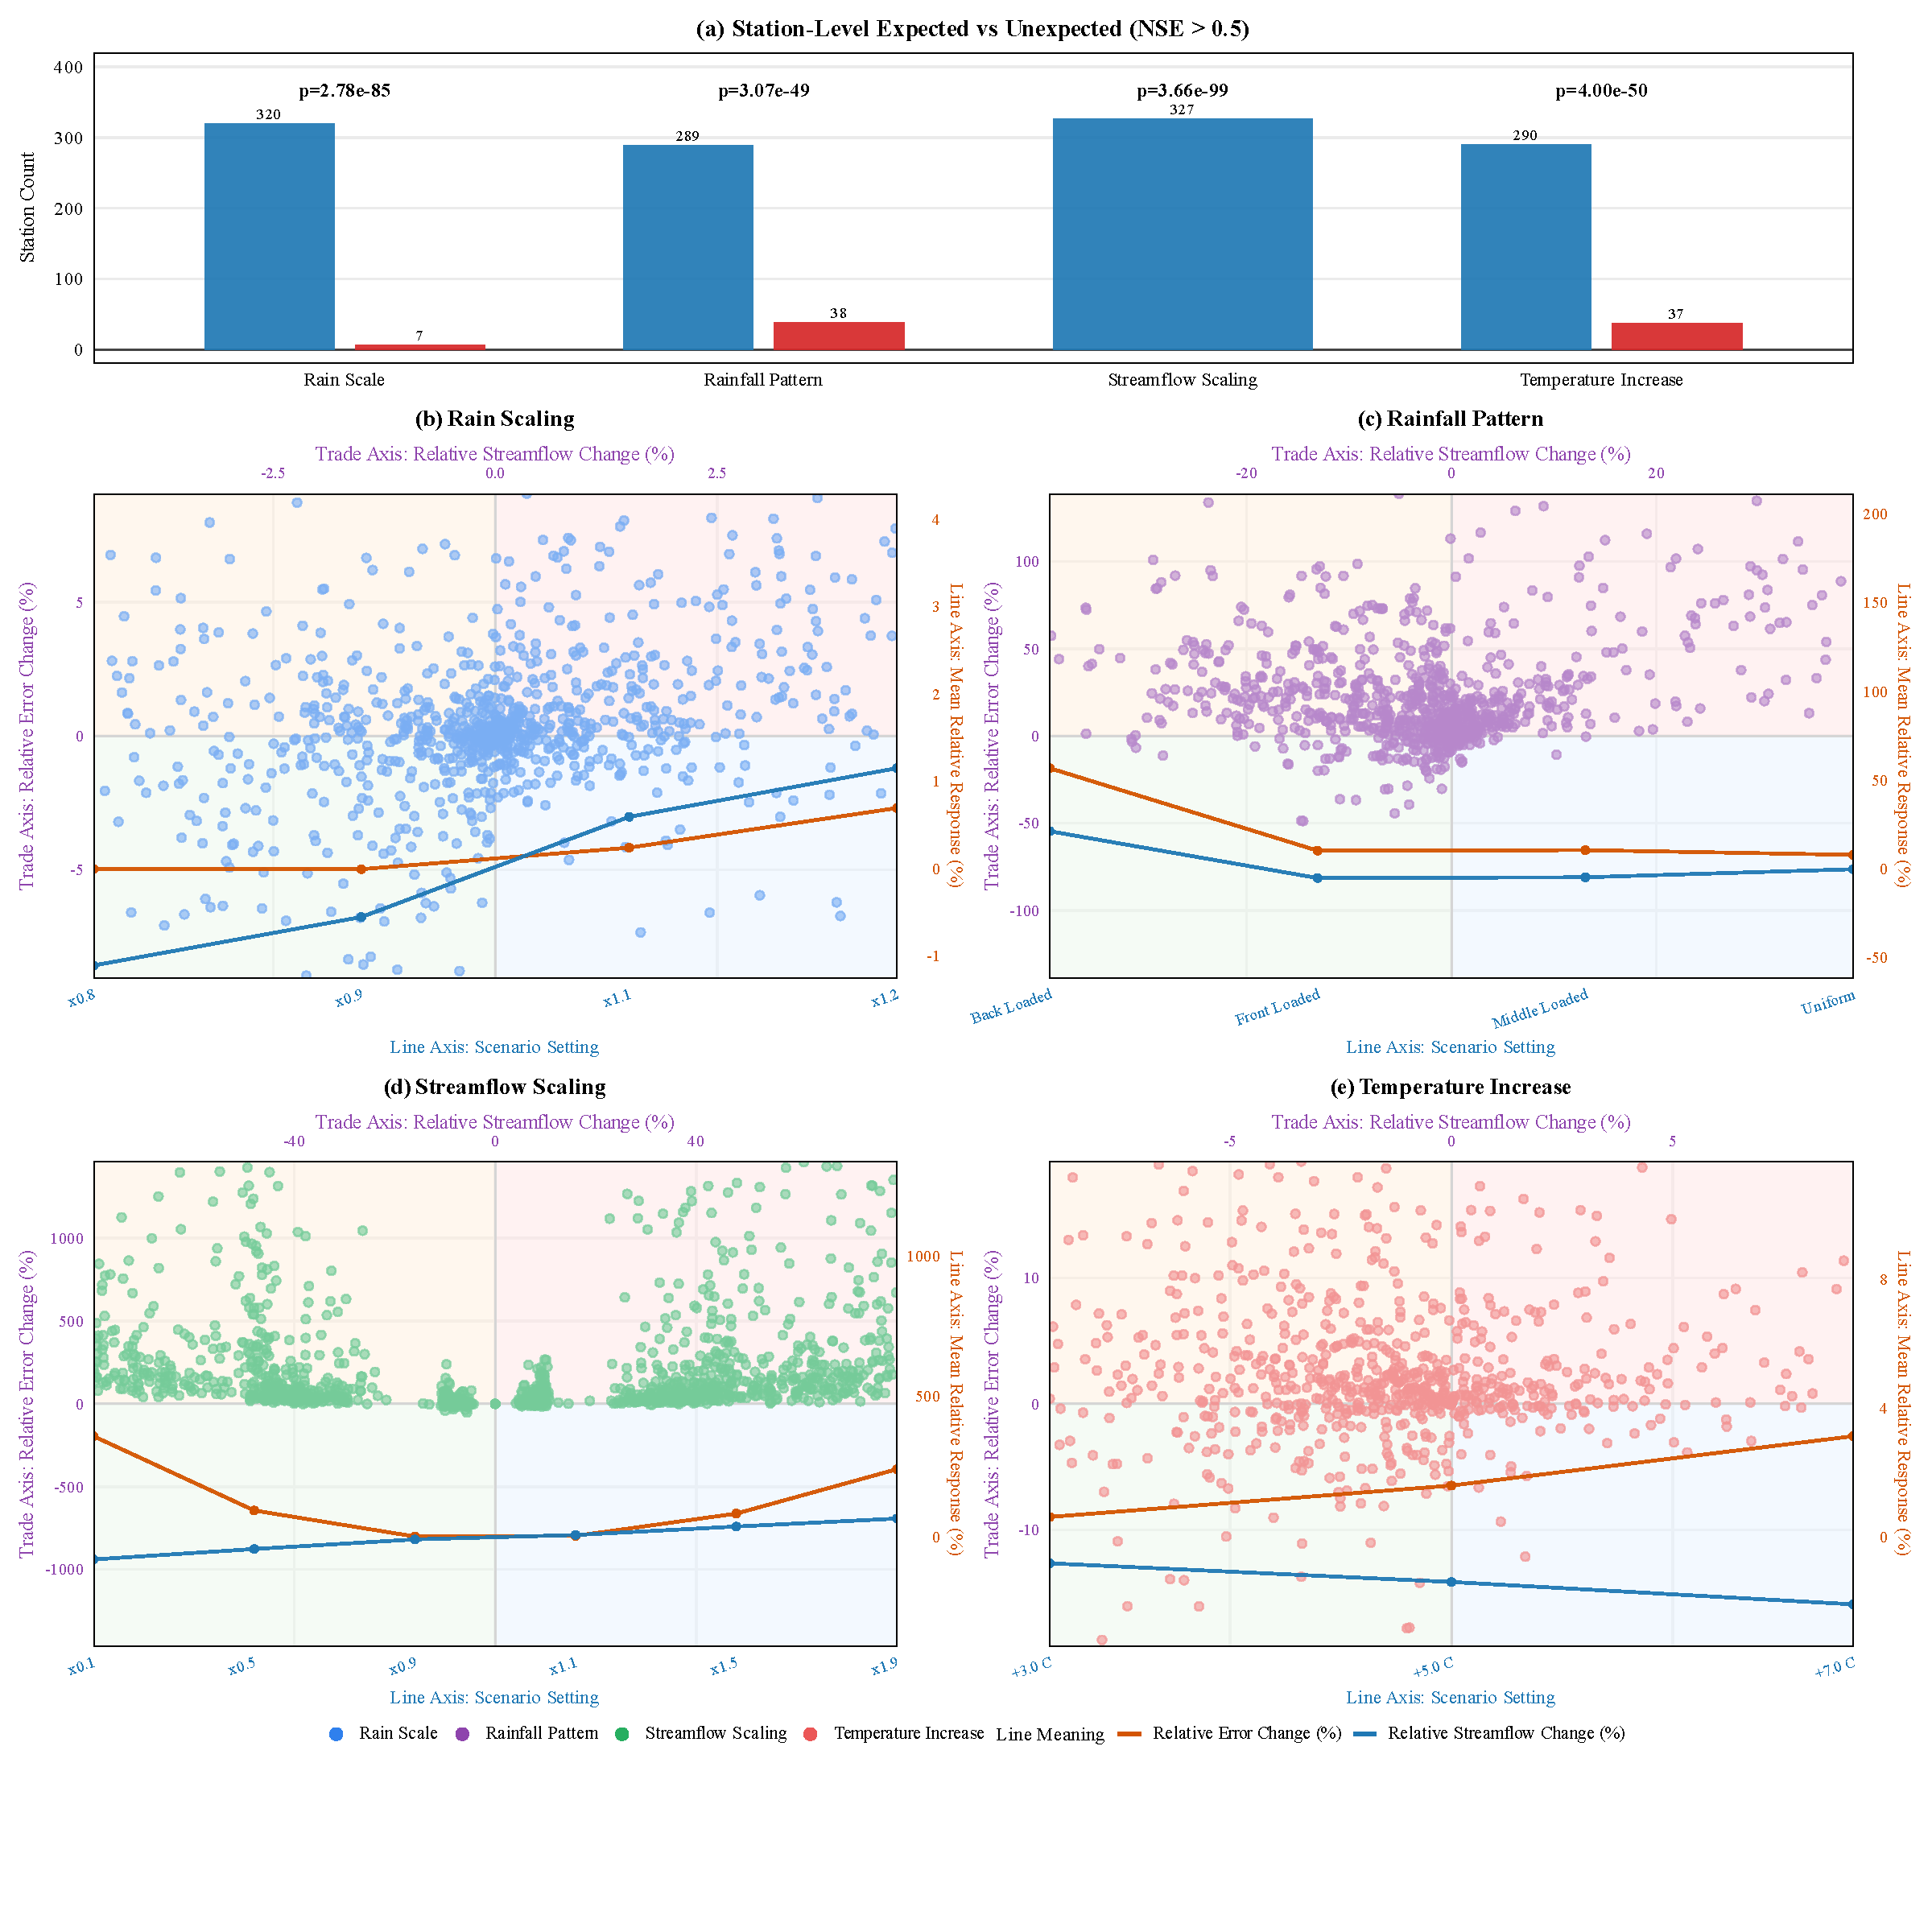
\includegraphics[width=\textwidth]{Figures/Fig_counterfactual_panel_main.pdf}
    \caption{\textbf{Counterfactual sensitivity analysis across intervention types. }(a) Station-level expected behavior statistics. (b) Rainfall scaling. (c) Rainfall pattern redistribution. (d) streamflow-state scaling. (e) Temperature perturbation.
        Blue lines denote relative changes in predicted streamflow volume, and orange lines denote relative changes in prediction error. Detailed experimental design and evaluation metrics are provided in Supplementary Information \ref{sec:sensitive}
    }
    \label{fig:counterfactual_main}
\end{figure}

\FloatBarrier

For streamflow-state perturbations (Fig.~\ref{fig:counterfactual_main}d), moderate scaling of recent streamflow history leads to corresponding adjustments in predicted volume, while prediction error remains stable. This demonstrates that the model can effectively utilize state information while maintaining consistent predictive performance. As the scaling magnitude increases, however, the model response gradually saturates, with volume changes no longer increasing proportionally to the input. This attenuation behavior indicates that the model does not simply amplify streamflow magnitude linearly, but instead imposes constraints on non-structured or inconsistent input variations, thereby avoiding unrealistic over-amplification. Such behavior suggests that the model captures streamflow dynamics through interactions among multiple hydrological factors\cite{bloschl2017changing} rather than relying solely on absolute magnitude.

For temperature perturbations (Fig.~\ref{fig:counterfactual_main}e), the predicted streamflow volume shows a slight decreasing trend, with consistent direction across snow-dominated and rainfall-dominated catchments and no significant difference between groups. This aligns with hydrological expectations that warming generally reduces streamflow through enhanced evapotranspiration or phase-related processes. In contrast, prediction error exhibits significantly different sensitivities between the two regimes: snow-dominated catchments show substantially stronger responses to temperature changes than rainfall-dominated ones\cite{milly2020colorado}, and this difference is consistent across warming magnitudes (p < 0.001). This suggests that the model not only captures the overall volumetric effects of temperature, but also differentiates between distinct hydrological knowledge patterns, reflecting sensitivity to process heterogeneity.

Overall, the model demonstrates robust responses to precipitation-driven volume changes and shows sensitivity to temporal structure and catchment state variations\cite{LouiseSlater2024_XAI_Hydrology}, indicating effective learning of key hydrological knowledge. At the same time, the differing response patterns across perturbation types suggest that the representation of more complex processes, such as temporal organization and state evolution, remains an area for further improvement. This behavioral consistency supports the validity of the extracted knowledge, and naturally leads to the final question: \textit{can this knowledge be transferred to improve other model classes?}


\subsection{Cross-Model Transfer Validates STEH-Derived Knowledge}

To answer this final question, we evaluate transferability using an external model family. Specifically, we designed a comparative experiment in which STEH-derived structural information is incorporated into a conventional Random Forest model\cite{Stephan2015} and compared against a baseline model without such information. The key purpose is not only to improve another model, but to test whether the extracted structures represent model-independent hydrological knowledge that remains effective outside the Transformer architecture\cite{song2026physics}. 

Furthermore, station-wise paired significance tests (paired t-test and Wilcoxon signed-rank test) demonstrate that the modified model significantly outperforms the baseline in a statistical sense, confirming the robustness of the observed improvements. Detailed descriptions of the model architecture, feature construction, and training and evaluation procedures are provided in Supplementary Information \ref{sec:rfDesign}.

From an overall perspective, the modified model exhibits consistent performance improvements across all stations\cite{li2024application}. Specifically, the NSE increases from 0.760 to 0.767, accompanied by reductions in both MSE and MAE, indicating enhanced predictive accuracy and error control\cite{WRR_MAE}. The station-wise comparison (Fig.~\ref{fig:rf_comparison}(d)) shows that most points lie above the diagonal line, suggesting that the modified model outperforms the baseline in the majority of cases. In addition, the improvement is observed across a wide range of baseline performance levels (Fig.~\ref{fig:rf_comparison}(e)), indicating that the benefit is not confined to specific subsets of stations. Together, these results indicate that the transferred structures retain predictive value in an independent model class, which supports the claim that STEH extracts non-model-specific hydrological knowledge rather than architecture-specific heuristics\cite{kalasampath2025_XAI}.

\begin{figure}[htbp]
    \centering
    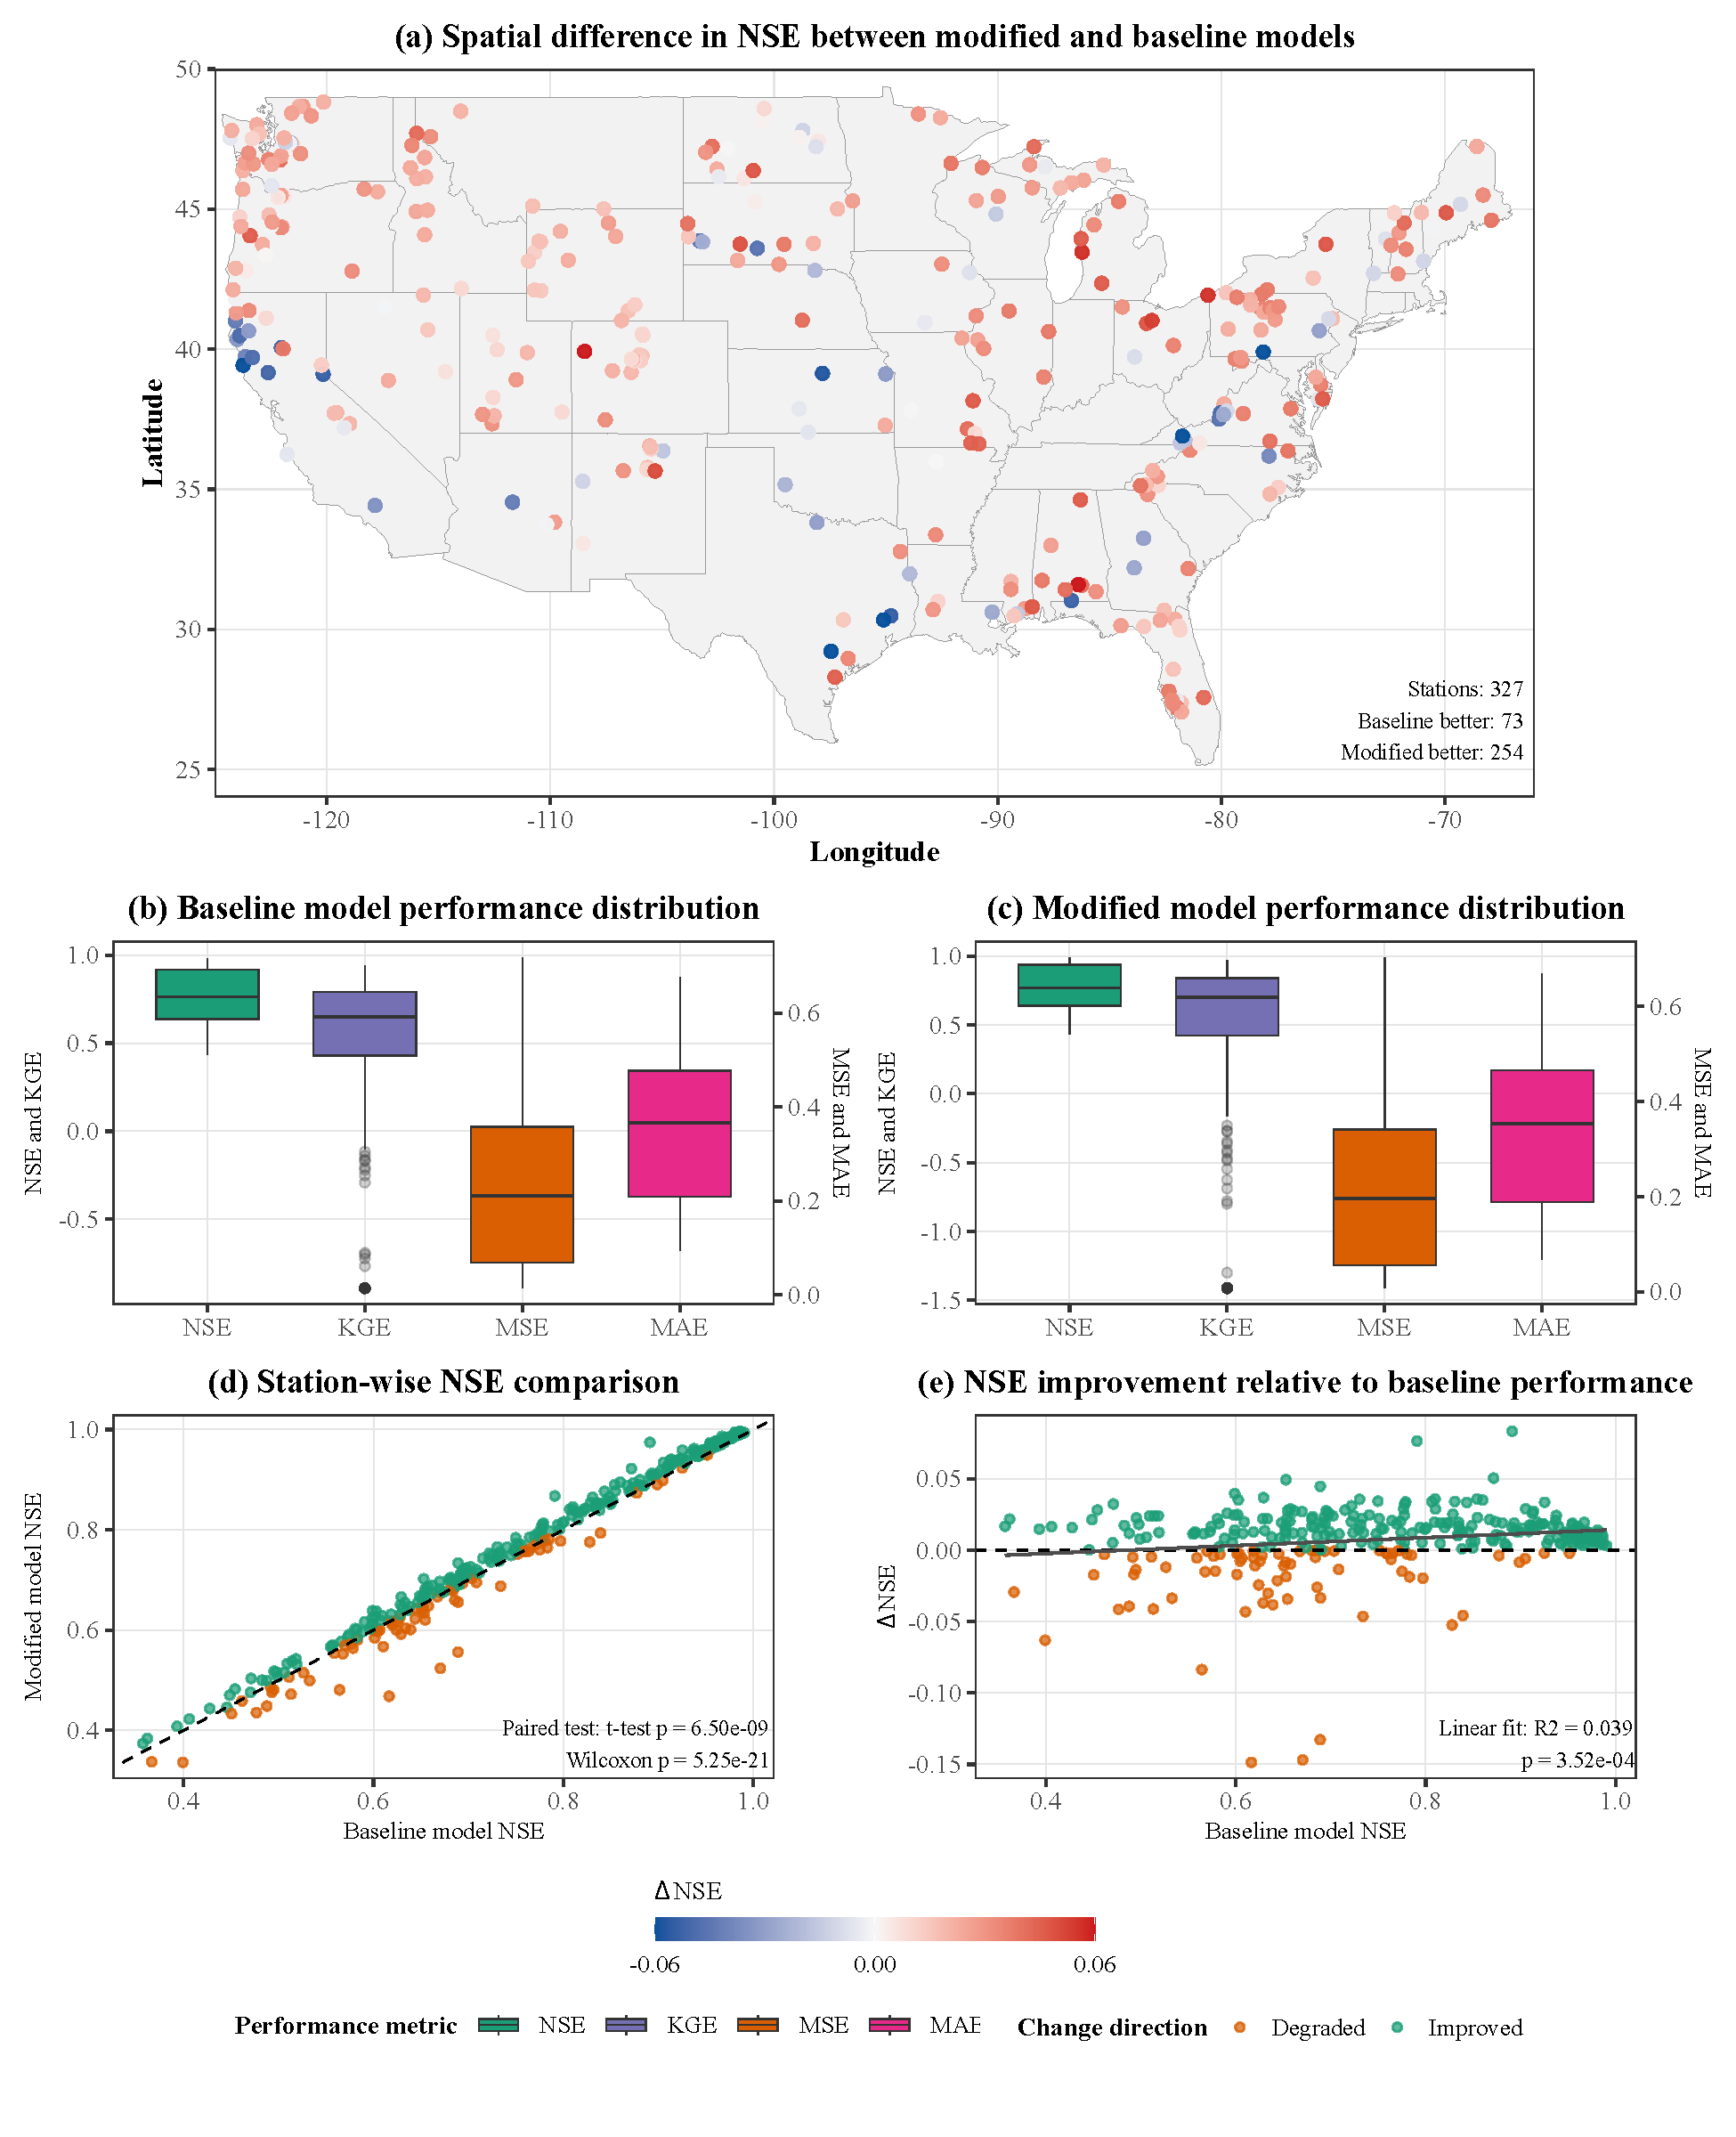
\includegraphics[width=\textwidth]{Figures/RF_Performance.pdf}

    \caption{
        \textbf{Performance comparison between baseline and STEH-informed Random Forest models.}(a) Spatial distribution of NSE differences (red: improved; blue: degraded).(b,c) Performance distributions of the baseline and modified models.(d) Station-wise NSE comparison (points above the diagonal indicate improvement).(e) NSE improvement relative to baseline performance.All results are based on stations with STEH model performance (NSE $>$ 0.5).
    }

    \label{fig:rf_comparison}
\end{figure}

\begin{table}[htbp]
    \centering
    \begin{threeparttable}
        \caption{Performance comparison between baseline and STEH-informed modified Random Forest models across hydro-climatic groups}
        \begin{tabular*}{\textwidth}{@{\extracolsep{\fill}}llccc}
            \toprule
            Model & Group & MSE & MAE & NSE \\
            \midrule

            \multirow{4}{*}{Baseline}
            & Arid          & 0.140054 & 0.260355 & 0.841540 \\
            & Humid         & 0.324556 & 0.435797 & 0.700072 \\
            & Sub-humid     & 0.270571 & 0.385097 & 0.724154 \\
            & All Stations  & 0.237974 & 0.353715 & 0.759683 \\

            \midrule

            \multirow{4}{*}{Modified}
            & Arid          & 0.133525 & 0.248404 & 0.846403 \\
            & Humid         & 0.313798 & 0.425727 & 0.709464 \\
            & Sub-humid     & 0.259417 & 0.372654 & 0.733143 \\
            & All Stations  & 0.228561 & 0.342049 & 0.767310 \\

            \bottomrule
        \end{tabular*}

        \begin{tablenotes}
            \footnotesize
            \item All metrics are averaged across stations within each hydro-climatic group. Only stations with STEH model performance (NSE $>$ 0.5) are included, as the extracted hydrological structures are derived from the STEH model and may become unreliable when its predictive performance is low.
        \end{tablenotes}

        \label{tab:rf_performance}
    \end{threeparttable}
\end{table}

Across different hydro-climatic regimes, the most pronounced improvements are observed in arid regions. As shown in Fig.~\ref{fig:rf_comparison}(a) and Table~\ref{tab:rf_performance}, inland arid and semi-arid areas exhibit predominantly positive performance gains. In the Arid group, the modified model consistently outperforms the baseline in terms of MSE, MAE, and NSE, indicating that the incorporation of structural information significantly enhances predictive capability under such conditions. This suggests that in environments where precipitation signals are weak and hydrological responses are governed by multiple interacting factors\cite{TAKEFUJI2025123514}, the inclusion of additional structural features enables the model to better capture streamflow dynamics.

In humid regions, the modified model also achieves consistent improvements (NSE: 0.700 to 0.709), although the magnitude of improvement is relatively smaller. This can be attributed to the comparatively simpler hydrological processes in such regions\cite{hess-25-2997-2021}, where streamflow generation is primarily controlled by a dominant driver. Under these conditions, the baseline model is already capable of capturing the main dynamics, leaving limited room for further improvement. Nevertheless, the continued reduction in error metrics indicates that structural information still contributes to improved fine-scale representation\cite{ABBASI2021125717}.

Overall, these findings demonstrate that the structural information extracted by STEH is not only interpretable but also scientifically verifiable through cross-model transfer. In particular, in regions characterized by complex or multi-factor-controlled processes, incorporating such structural knowledge can substantially improve model performance. More importantly, successful transfer to Random Forest provides an external validation step: the extracted knowledge is not tied to a single network design, but reflects portable hydrological regularities. This transfer result closes the full evidence chain of this section: hydrological knowledge is broadly encoded across models, its content can be structurally identified, its physical consistency can be behaviorally validated, and its non-model-specific validity can be verified through cross-model transfer.

\FloatBarrier